\documentclass[10pt]{article}
\usepackage[utf8]{inputenc}

\usepackage{graphicx} % Required for inserting images
\usepackage{multicol}
\usepackage{wrapfig}
\usepackage{float}

\usepackage{hyperref}
\usepackage{svg}
\usepackage{subfig}
\usepackage{siunitx}

\usepackage[%
    a4paper,
    top=1.2cm,
    bottom=1.6cm,
    left=1.8cm,
    right=1.8cm,
    marginparwidth=1.75cm
]{geometry}

\title{RS: Second Homework}
\author{
    Mark Loboda in Simon Goričar
}
\date{19. 4. 2025}

\begin{document}
\maketitle

\section{Benchmarks}

\subsection{First task: performance of a snooping-based cache coherence protocol}
In this task, we ran the Cholesky decomposition workload using \texttt{GEM5} and observed several metrics related to the snooping-based cache coherence protocol in a multiprocessor system. We benchmarked systems with $2$, $4$, $8$, and $16$ processors, each one with $32~\text{KiB}$ of 8-way associative L1 cache and $256~\text{KiB}$ of 8-way associative L2 cache; we used $2~\text{MiB}$ of 16-way associative global L3 cache.


\begin{figure*}[htbp]
    \centering
    \subfloat[Per-core CPI against number of CPUs.]{%
        \includesvg[width=0.4\linewidth]{images/task1/per-core-cpi-against-number-of-cpu.svg}
        \label{fig:task1:per-core-cpi}
    }\hfill
    \subfloat[Per-core L1 miss rate against number of CPUs.]{%
        \includesvg[width=0.4\linewidth]{images/task1/per-core-l1-miss-rate-against-number-of-cpu.svg}
        \label{fig:task1:per-core-l1-miss-rate}
    }\\
    
    \subfloat[L3 upgrade requests against number of CPUs.]{%
        \includesvg[width=0.4\linewidth]{images/task1/l3-upgrade-requests-against-number-of-cpus.svg}
        \label{fig:task1:l3-upgrades}
    }\hfill
    \subfloat[Snoop traffic against number of CPUs.]{%
        \includesvg[width=0.4\linewidth]{images/task1/snoop-traffic-against-number-of-cpus.svg}
        \label{fig:task1:snoop-traffic}
    }\\

    \caption{Results of our snooping-based cache coherence protocol benchmark.}
    \label{fig:task1}
\end{figure*}

First off, let's have a look at how the average and per-core \textbf{cycles per instruction} (CPI) values are impacted by different numbers of processors (figure \ref{fig:task1:per-core-cpi}). As we can see on the plot, the CPI of the primary processor stays rather fixed, but each subsequent core observes a lower CPI, with a 16-CPU system having the smallest of all tested configurations. It's hard to say precisely why, but our guess is that, since cores other than the first one are usually part of OpenMP's worker thread pool, the work those threads execute is commonly numeric, focused, and uses heavily optimized operations or instructions (or a \texttt{for} loop with rather simple computations, which the compiler may be able to optimize well). This could also mean that the branch predictions for those focused short operations, if any, are more often correct, leading to a lower average cycles per instruction value.

Secondly, let's look at the \textbf{L1 miss rate}, both on average and per core (figure \ref{fig:task1:per-core-l1-miss-rate}). As we can see in the figure, the higher the number of CPUs in the system, the larger the L1 miss rate of the primary core; the likely reason is that the primary core belongs to the main thread, whose goal is to execute the entire program, not just the focused computations (which the rest of the cores mostly do). If we assume that, we can conclude that the work the rest of the cores do is limited in the number of instructions and often repeated (e.g., in a \texttt{for} loop), leading to a rather small instruction cache requirement compared to the first core, which has to go through the entire program.

Thirdly, \textbf{L3 upgrade requests} and \textbf{snoop traffic} (figures \ref{fig:task1:l3-upgrades} and \ref{fig:task1:snoop-traffic}). Here we simply observe that the number of L3 cache upgrade requests and the presence of snoop traffic grow as the number of cores on the system increases, seemingly linearly. The increasing number of L3 cache upgrades could come from the higher number of cores having to compete for an upgraded cache line on their core more often (for cases where two or more cores need to write to the same cache line, even if not to the same value). The increase in snoop traffic is also very sensible, as the cache coherence mechanisms have much more work to do as the number of coherent cores to maintain gets higher.


\subsection{Second task: Impact of false sharing on performance in directory-based cache coherence protocols}
In this task, we examined the impact of false sharing on a parallelized program for computing digits of $\pi$. Two program versions were compared: the first with false sharing present, where multiple threads share a cache line, and the second, where the program is optimized to avoid this issue. False sharing can lead to unnecessary cache line invalidations and increase memory traffic.

We used \texttt{GEM5} configured with the SMP Ruby coherence protocol and two versions of the workload. Additionally, we used $32~\textbf{KiB}$ of 8-way associative L1 cache and $256~\text{KiB}$ of 8-way associative L2 cache, both with 64-byte cache lines. We measured the performance using $2$, $4$, $8$, and $16$ processors.

\begin{figure*}[htbp]
    \centering
    \subfloat[]{%
        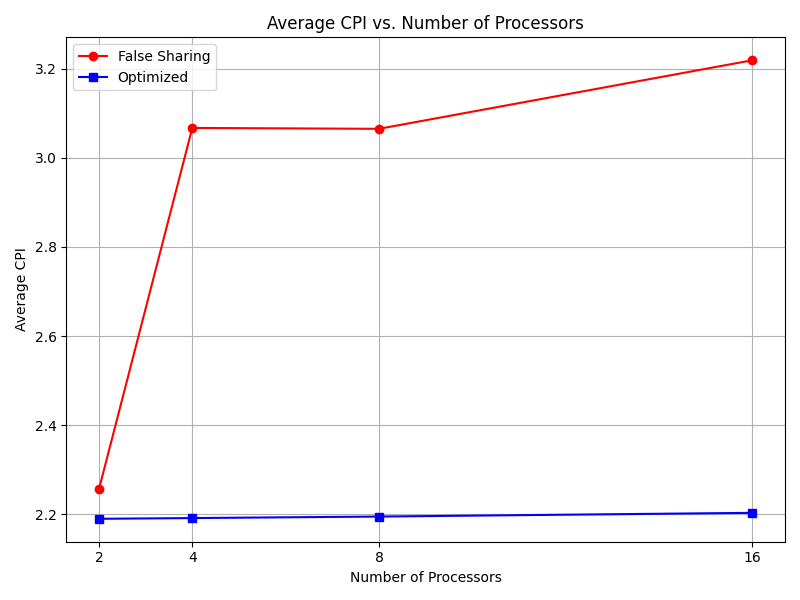
\includegraphics[width=0.42\linewidth]{images/task2/cpi_plot.png}
        \label{fig:task2:cpi}
    }\hfill
    \subfloat[]{%
        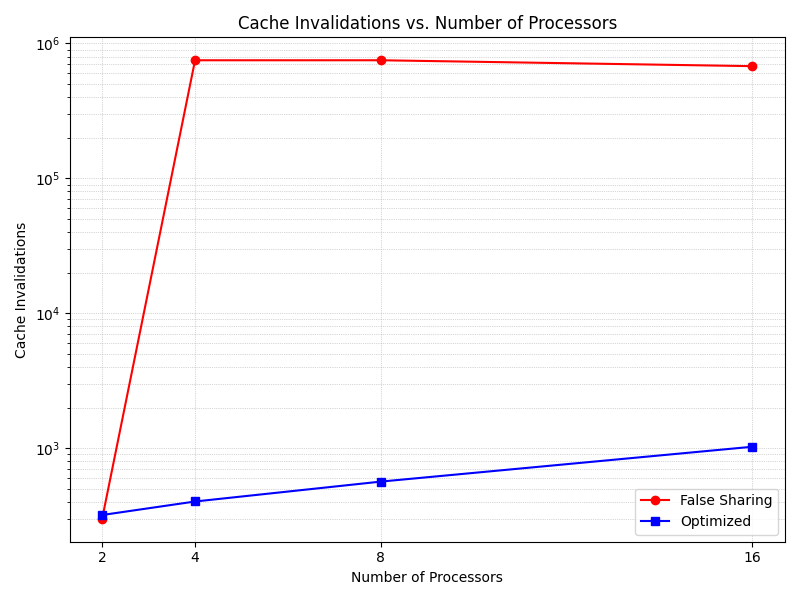
\includegraphics[width=0.42\linewidth]{images/task2/cache_invalidation_plot.png}
        \label{fig:task2:cache_invalidations}
    }\\
    \caption{Results of our false sharing benchmark.}
    \label{fig:task2:fig1}
\end{figure*}

We noticed that the CPI of the false sharing implementation is substantially higher as the number of processors increases, while the optimized version's CPI stays relatively the same (figure~\ref{fig:task2:cpi}). This is likely to be in large part due to the number of cache invalidations occurring in the workload with false sharing, meaning a larger number of cycles is spent reloading cache lines (figure~\ref{fig:task2:cache_invalidations}). The problem is compounded as the number of processors increases because more cores continuously fight over shared cache lines.

We also analyzed the memory coherence behavior of the two workloads by looking at the number of L1 load operations across the four MESI states: \textbf{Modified}~(M), \textbf{Exclusive}~(E), \textbf{Shared}~(S) and \textbf{Invalid}~(I).

\begin{figure*}[htbp]
    \centering
    \subfloat[]{%
        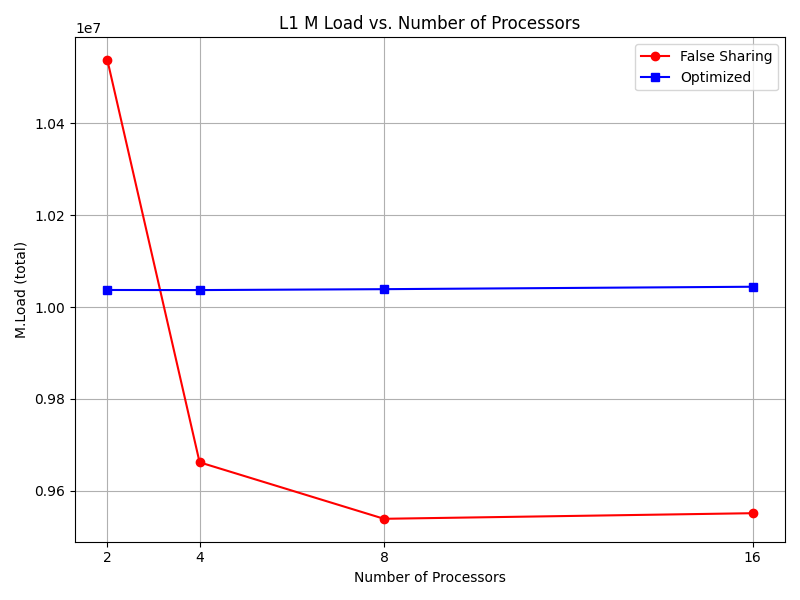
\includegraphics[width=0.47\linewidth]{images/task2/load_M_plot.png}
        \label{fig:task2:m_load}
    }\hfill
    \subfloat[]{%
        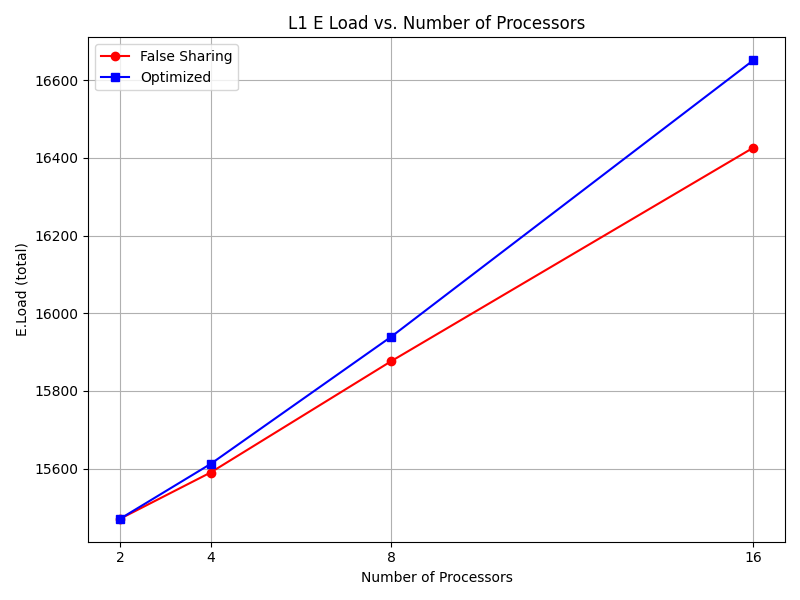
\includegraphics[width=0.47\linewidth]{images/task2/load_E_plot.png}
        \label{fig:task2:e_load}
    }\\
    \subfloat[]{%
        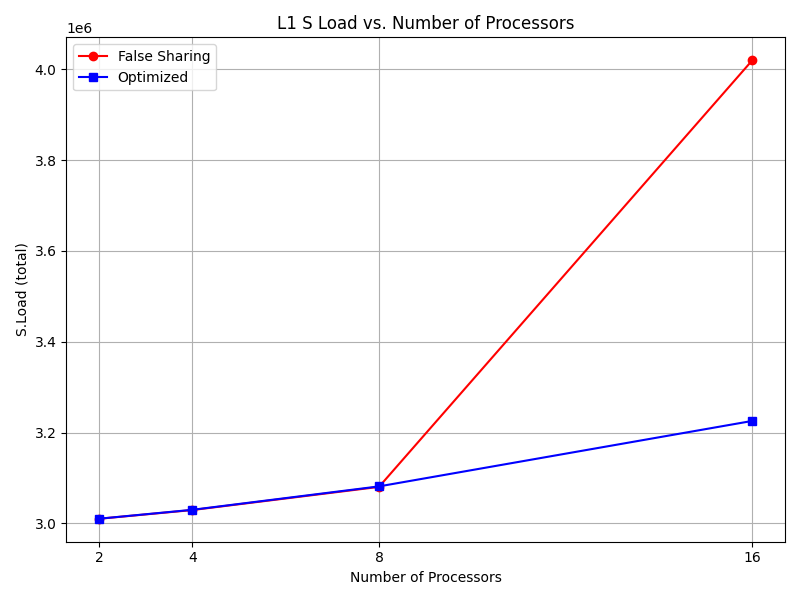
\includegraphics[width=0.47\linewidth]{images/task2/load_S_plot.png}
        \label{fig:task2:s_load}
    }\hfill
    \subfloat[]{%
        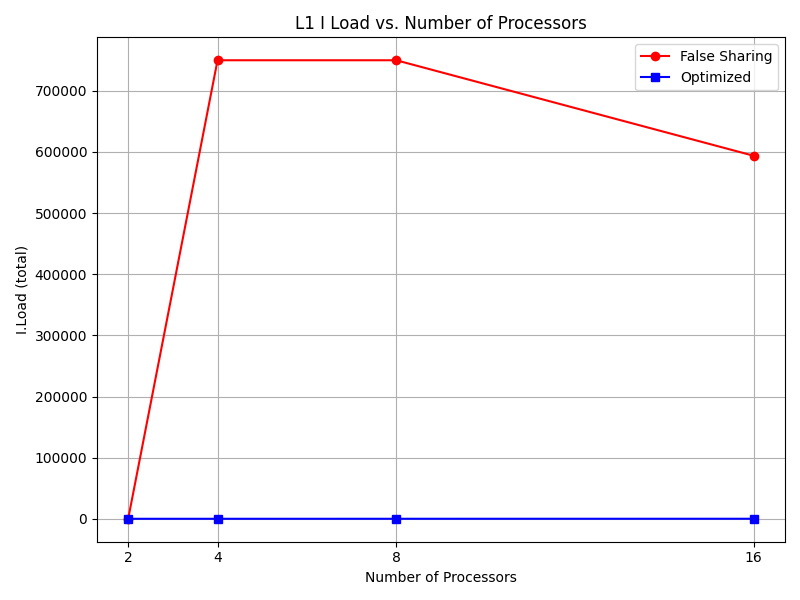
\includegraphics[width=0.47\linewidth]{images/task2/load_I_plot.png}
        \label{fig:task2:i_load}
    }\\
    \caption{Results of the pi integration benchmark of the number of loads under different states.}
\end{figure*}

The measured values clearly differ between implementations of the two integration workloads. \textbf{I-state} loads are significantly higher in the false sharing algorithm, as the false sharing causes frequent cache line invalidations, forcing cores to reload frequently. The optimized version shows consistently lower loads in the I-state. Operations in the \textbf{S-state} only deviate with sixteen processors, where the optimized algorithm shows a more stable and efficient scaling of the number of processors. The number of \textbf{E-states} scales consistenly with the number of processors but is more frequent in the optimized algorithm, suggesting an improved handling of non-shared data. When looking at the \textbf{M-states}, the optimized algorithm displays a consistent number across all numbers of processors, while the false sharing only shows a high number with two cores but quickly falls off when scaling to more cores. We conclude that the optimized version of the algorithm improves utilization of the cache hierarchy and the MESI protocol, improving efficiency.

\begin{figure}[hbtp]
    \centering
    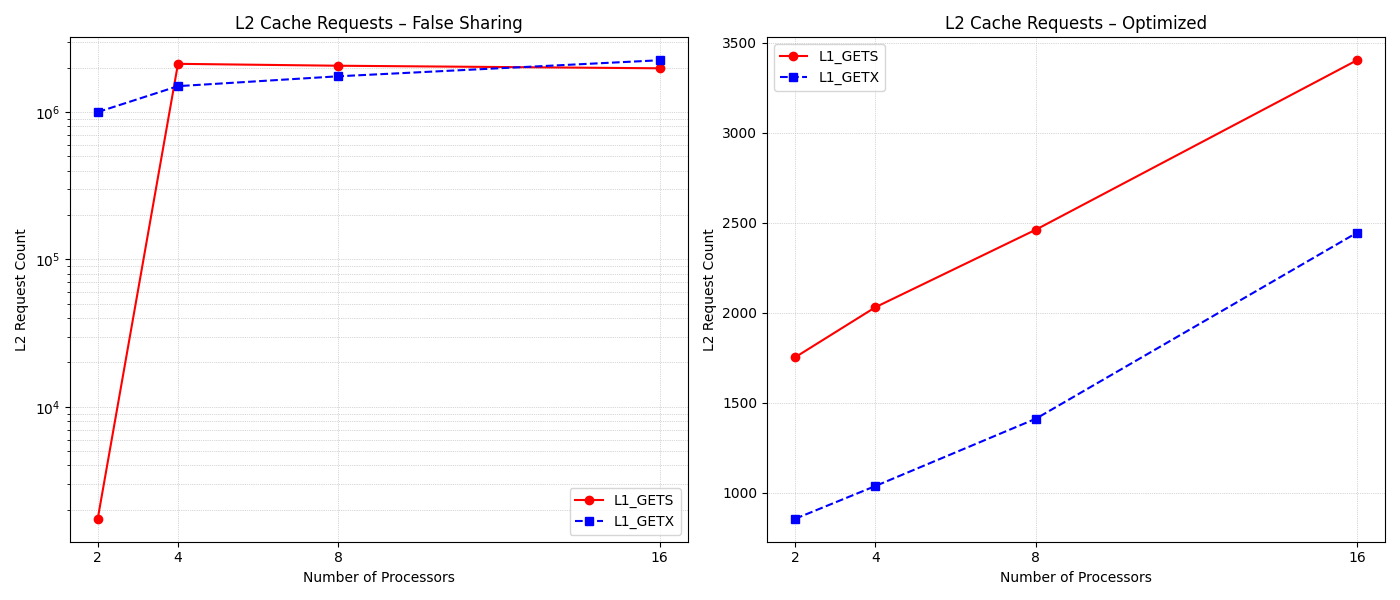
\includegraphics[width=0.82\linewidth]{images/task2/l2_requests_plot.png}
    \caption{L2 requests with two implementations of the workload.}
    \label{fig:task2:l2_requests}
\end{figure}

The data for the L2 cache requests~\ref{fig:task2:l2_requests} in the false sharing algorithm shows significantly more \texttt{GETS} and \texttt{GETX} requests compared to the optimized version. The implementation with false sharing causes increased memory traffic due to frequent cache invalidations and data reloads.

\begin{figure}[hbtp]%{r}{0.65\textwidth}
    \centering
    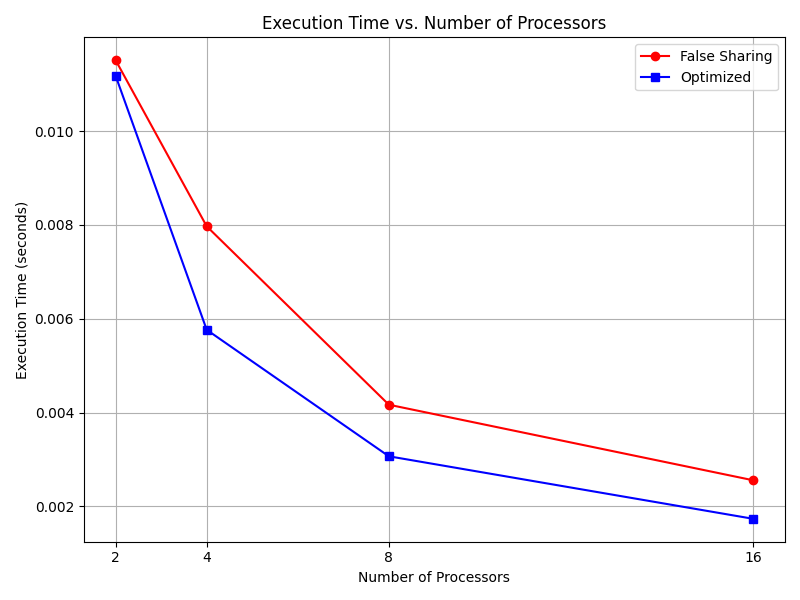
\includegraphics[width=0.4\linewidth]{images/task2/execution_times_plot.png}
    \caption{Execution times of the two implementations across different processor counts.}
    \label{fig:task2:exec_time}
\end{figure}

To conclude, we can see that the optimized version improves on cache line invalidations that otherwise occur with the false sharing implementation. It also increases memory traffic with L2 cache \texttt{GETS} and \texttt{GETX} requests. This affects the CPI and overall execution time (figure~\ref{fig:task2:exec_time}) when running both algorithms.



\subsection{Third task: performance of different interconnection networks}
In this task, we ran the STREAM benchmark and observed several metrics related to the traffic on the interconnection network. We benchmarked systems with $2$, $4$, $8$, and $16$ processors, $32~\text{KiB}$ of 8-way associative L1 cache, and $256~\text{KiB}$ of 8-way associative L2 cache.

\begin{figure*}[htbp]
    \centering
    \subfloat[Network messages against number of CPUs in system for \textit{crossbar} interconnection network.]{%
        \includesvg[width=0.4\linewidth]{images/task3/message-counts-against-number-of-cpu-for-crossbar.svg}
        \label{fig:task3:crossbar}
    }\hfill
    \subfloat[Network messages against number of CPUs in system for \textit{point-to-point} interconnection network.]{%
        \includesvg[width=0.4\linewidth]{images/task3/message-counts-against-number-of-cpu-for-point-to-point.svg}
        \label{fig:task3:point-to-point}
    }\\
    
    \subfloat[Network messages against number of CPUs in system for \textit{ring} interconnection network.]{%
        \includesvg[width=0.4\linewidth]{images/task3/message-counts-against-number-of-cpu-for-ring.svg}
        \label{fig:task3:ring}
    }\hfill\\

    \caption{Results of our interconnection network benchmark.}
    \label{fig:task3}
\end{figure*}

As we can see in figures \ref{fig:task3:crossbar}, \ref{fig:task3:point-to-point}, and \ref{fig:task3:ring}, the number of messages exchanged on the interconnection network monotonically grows as the number of cores in the system increases. The increase is least visible on the \textit{crossbar} and \textit{point-to-point} network topology, likely because in those two network types, the messages that need to be exchanged perform the minimal number of hops needed to reach their destination (1 hop in the case of point-to-point and about two hops in the case of crossbar). The somewhat linear increase is visible on the \textit{ring} network because, as the number of cores increases, so does the number of average hops required to send a message to the core you want (it's rather unlikely the target core will be next in the chain).


% \end{multicols}

\end{document}
